

\documentclass[../../e1_tp1_main.tex]{subfiles}

\begin{document}
\chapter{Circuito con diodo}

El circuito estudiado en esta secci\'on es el siguiente:

\begin{figure}[H]
\centering
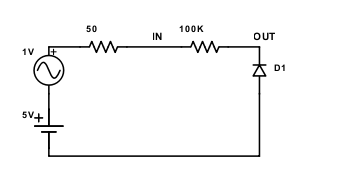
\includegraphics[width=0.5\textwidth]{imagenes/cirq.png}
\caption{Esquema del circuito}
\end{figure}


\section{Modelo del diodo en AC}

El diodo en corriente alterna, con pequeñas amplitudes, se puede modelar como el paralelo de un capacitor con una resistencia. La resitencia es la din\'amica del diodo, la cual se mantiene constante debido a la baja amplitud de entrada. En cuanto a la capacidad, \'esta proviene de dos fen\'omenos distintos: la capacidad de difusi\'on y la proveniente de la juntura. Esta \'utlima se debe a que la juntura se puede modelar como un diel\'ectrico separando dos superficies con carga opuesta.

\begin{figure}[H]
\centering
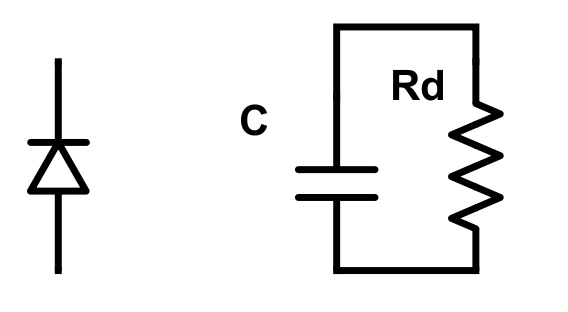
\includegraphics[width=0.5\textwidth]{imagenes/modAc.png}
\caption{Modelo AC del diodo}
\end{figure}

\section{Funci\'on transferencia}

Teniendo en cuenta el modelo del diodo, y aplicando un divisor de tensión, se obtiene la funci\'on transferencia del circuito:

\begin{equation}
H(s)= \left(\frac{R_D}{R + R_D} \right) \cdot \left( \frac{1}{1+ \frac{s}{\left(\frac{R+R_D}{C R_D}\right)}}\right)
\end{equation}

La funci\'on transferencia hallada corresponde a un sistema de primer orden. Como la parte real de su polo es negativa, el sistema es BIBO estable, y por lo tanto para hallar la respuesta en frecuencia basta evaluar $s=j\omega$. Esta funci\'on corresponde a un filtro pasabajos con frecuencia de corte $\omega_C = $ \todo{PONER LA FRECUENCIA DE CORTE}. Por ende, se esperar\'ia que para frecuencias mucho menores a $f_C = \frac{\omega_C}{2\pi}$ no haya atenuaci\'on, en $f = f_C$, la atenuaci\'on sea de $3dB$, y para $f\gg f_c$ se aten\'ue $20dB$ por d\'ecada. En cuanto a la fase, se esperaria que var\'ie entre $0^\circ$  y $-90^\circ$, pasando por $-45^\circ$ en la frecuencia de corte. \par

De la hoja de datos del 1N4007 obtuvimos que su capacitancia es de aproximadamente $8pF$.

\begin{figure}[H]
\centering
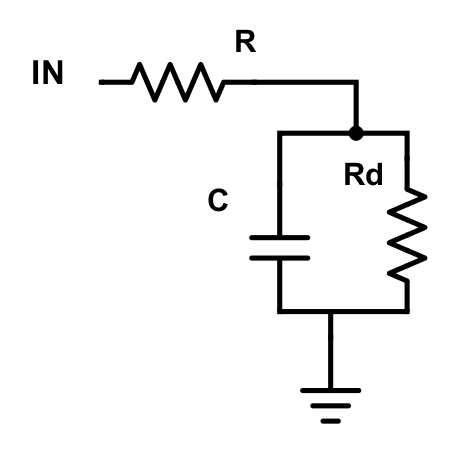
\includegraphics[width=0.45\textwidth]{imagenes/modCD.png}
\caption{Circuito con modelo AC del diodo}
\end{figure}
\section{Mediciones}

Las mediciones se realizaron con un generador de funciones y un osciloscopio, con las puntas configuradas en $\times 1$.

\begin{figure}[H]
\centering
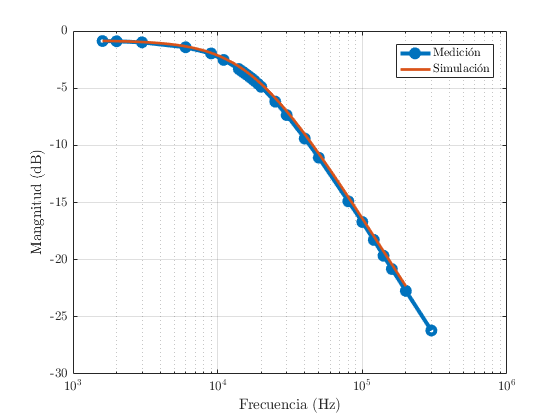
\includegraphics[width=0.75\textwidth]{imagenes/mag.png}
\caption{Magnitud de la respuesta en frecuencia, medida y simulada}
\end{figure}

\begin{figure}[H]
\centering
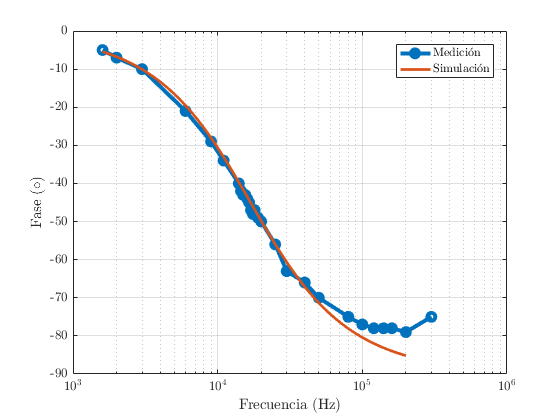
\includegraphics[width=0.75\textwidth]{imagenes/fase.png}
\caption{Fase de la respuesta en frecuencia, medida y simulada}
\end{figure}

\section{Conclusión}

Se observa en los gr\'aficos que la simulaci\'on se ajusta a las mediciones. Sin embargo, para que esto suceda en la simulaci\'on se tuvo que tener en cuenta los efectos de las puntas del osiloscopio, modeladas como el paralelo de un capacitor de $100pF$ con una resistencia de $1M \Omega$, alterando el comportamiento predicho. Adem\'as, $R_D$ no se puede considerar constante, debido a que el circuito se alimento con una tensi\'on  de $1V_{pp}$, con lo cual no se cumple con la premisa de amplitudes peque\~nas.

\end{document}

